%% wlkr
\documentclass[12pt,journal,compsoc]{IEEEtran}
\usepackage{graphicx}

\begin{document}
\title{Using Twitter Data and Sentiment Analysis to Predict Future Values of Cryprocurrencies}

\author{Ryan Walker}

\IEEEtitleabstractindextext{%
\begin{abstract}
This paper presents numerical schemes for gathering, processing and correlating sentiment data to actual cost 
for a given crypocurrency over a given unit of time in the interest in finding a time-lagged correlation. 
\end{abstract}
}

% make the title area
\maketitle
\IEEEpeerreviewmaketitle

\section{Introduction}
\IEEEPARstart{S}{entiment} analysis techniques have been used for stock market predictions in the past  with 
mixed success \cite{BI1}. We are of the opinion that for a technique like this to work there are three major requirements.

\begin{enumerate}
\item High volume of sentiment source
\item Strong correlation to trader action and community opinion
\item Low quantity of non-deterministic value changing artifacts news reports, earnings, company announcements, etc...
\end{enumerate}

In most cases, point one and three are mutually exclusive, meaning if there is a high volume of people talking about a
stock publicly $\frac{100k+}{Day}$, the company will typically be publishing earning reports, posting news, etc... 
These are important for investors, but cannot be accurately modeled as they are considered random artifacts.\\

As there are still news artifacts regarding Cryptocurrencies, they are less common and typically 
have less of an impact because unless there is a major problem with the algorithm, they are mostly subjective, unlike 
an earning report or other financial documents.\\

The aim of this paper is to attempt to validate what has been listed above, and use the data to make further informed 
buys and sells.

\subsection{Gathering Sentiment Data}
The main source of sentiment data was from twitter. A Python module \textit{tweepy} \cite{Tweepy} was used to gather
tweets and then bin them into cryptocurrencies of interest, the volume was anywhere from $1.2k \frac{tweets}{hr}$
to $24k \frac{tweets}{hr}$ depending on the currency of interest. For this paper we were mostly interest in BTC, as the
tweet volume is the highest, in the past five months, we have gathered over 21 billion tweets on Bitcoin alone.\\

Once the data is gathered it's put into a time series dataset with a period of 30 seconds - from that point Python \textit{NLTK} 
(Natural Language Toolkit) \cite{NLTK} is used to perform sentiment analysis to rate each tweet and make a net sum per unit time. 
Figure \ref{fig:RawSent} shows the output of what I have described above.

\begin{figure}[hp]
	\centering
	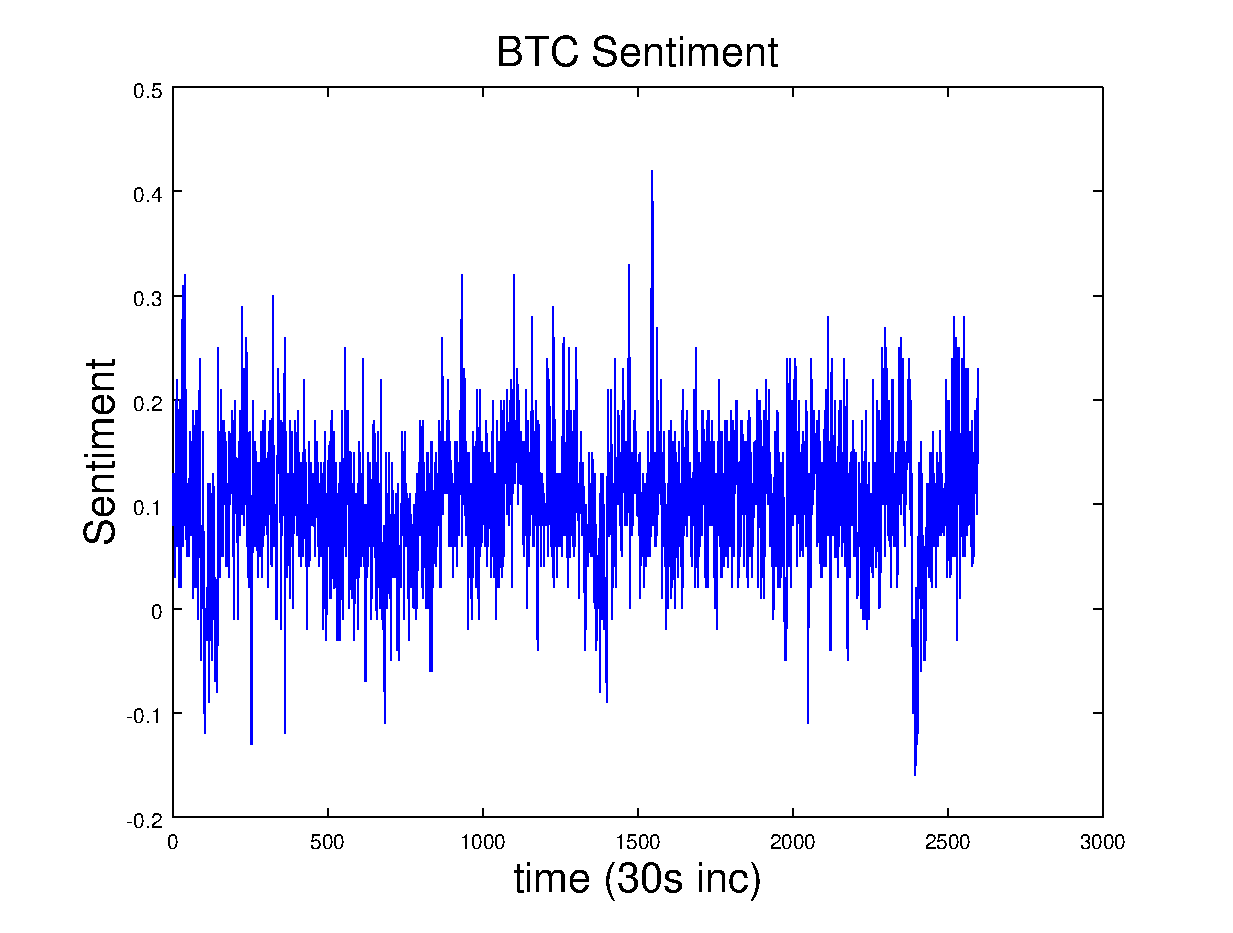
\includegraphics[width=0.5\textwidth]{../Datasets/Plots/Oct9_Sen}
	\caption{Raw Sentiment, October 9th 2017}
	\label{fig:RawSent}
\end{figure}

After a little filtering Figure \ref{fig:FilteredSent} - it's possible to compare the sentiment and values time series.

\begin{figure}[h]
	\centering
	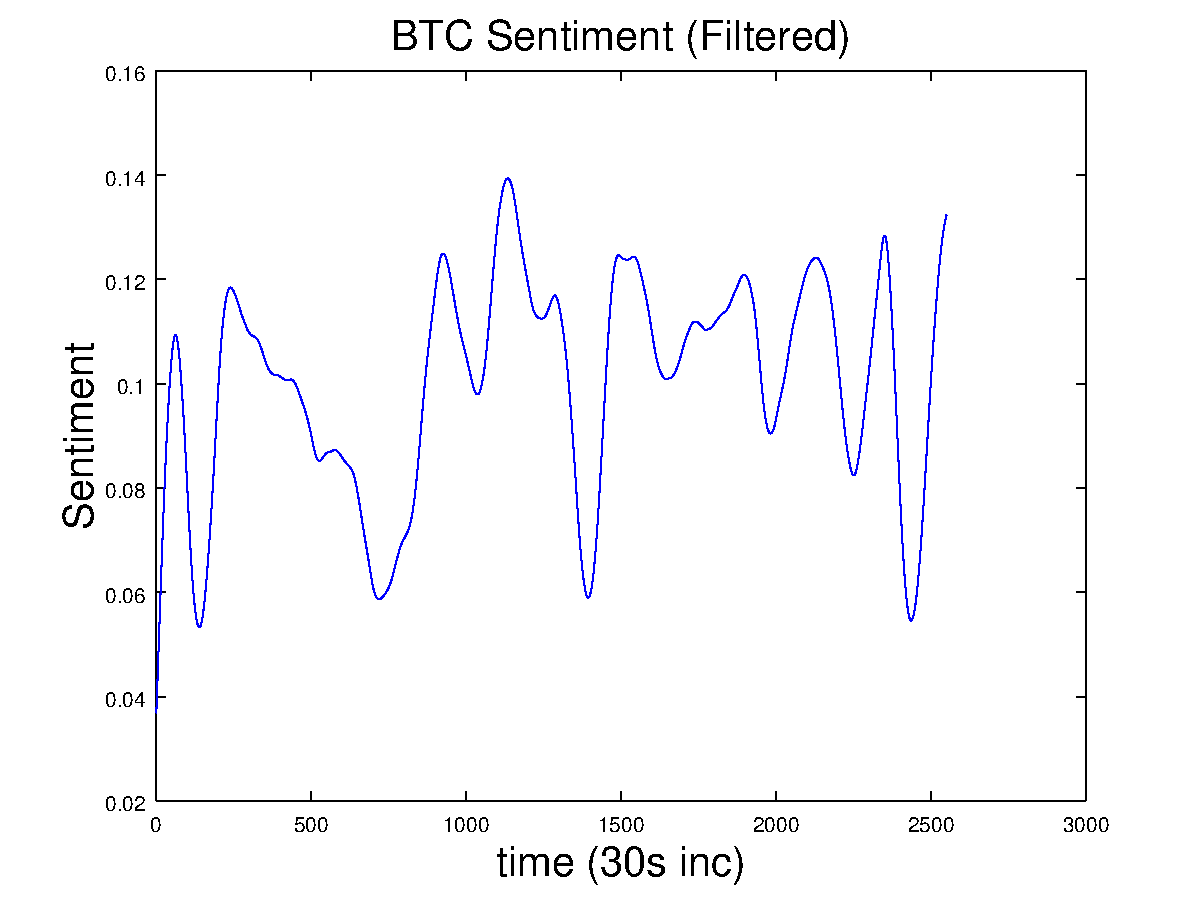
\includegraphics[width=0.5\textwidth]{../Datasets/Plots/Oct9_Sen_Fil}
	\caption{Filtered Sentiment, October 9th 2017}
	\label{fig:FilteredSent}
\end{figure}

\subsection{Timewise Correlation}
In the beginning, the plots were manually shifted forward in time until they 'looked right', later a numerical method was used
for correlation.\\

The timewise correlation was done by what we call the time correlation vector $k$ which is defined as equation \ref{eq:K}

\begin{equation}\label{eq:K}
k_j = \frac{\sum\limits_{i=0}^n x_i - y_{i+j}}{n-j} \textrm{, where j runs from 0 to n}
\end{equation}

\begin{figure}[h]
	\centering
	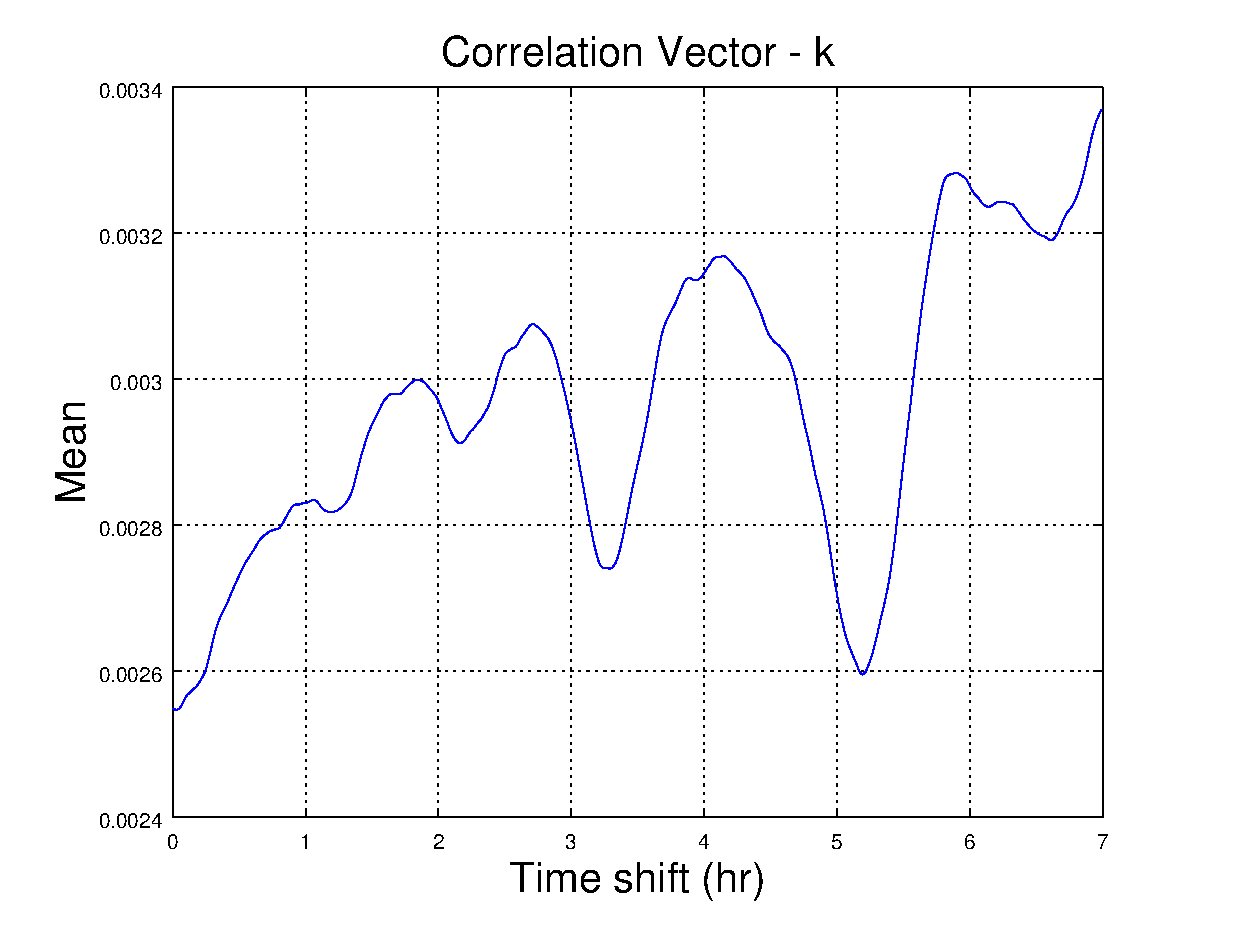
\includegraphics[width=0.5\textwidth]{../Datasets/Plots/Oct7_K}
	\caption{Time Correlation vector $k$, October 7th 2017}
	\label{fig:K}
\end{figure}

Where $x = \frac{dCost}{dt}$ $y = \frac{dSent}{dt}$, the reasoning for using derivatives for the correlation is simply because
the sentiment values are effectively a floating quantity - where the magnitude is not believed by us to have any direct 
relationship to the magnitude of cost. However, our findings have lead us to believe that a changing value of sentiment correlates
changing cost.\\

$k$ is a minimizing function where the lowest magnitude indicates the highest level of correlation between sentiment and cost.
As seen in Figure \ref{fig:K}, $k$ has a global minima around 5.2hrs, which I define as $\tau_L = 5.2hrs$ 
or the effective 'Time lag' between high values of changing sentiment and high values of changing cost.\\

It has been observed that $\tau_L$ has been repeatable over a given unit of time, Figure \ref{fig:Ksum} 
shows the vector sum of many $k$ from November 2nd to November 17th (15 $k$ vectors). In addition there are some interesting 
patterns appearing as local minama at $\sim1.8hrs$ and $\sim3.2hrs$.

\begin{figure}[h]
	\centering
	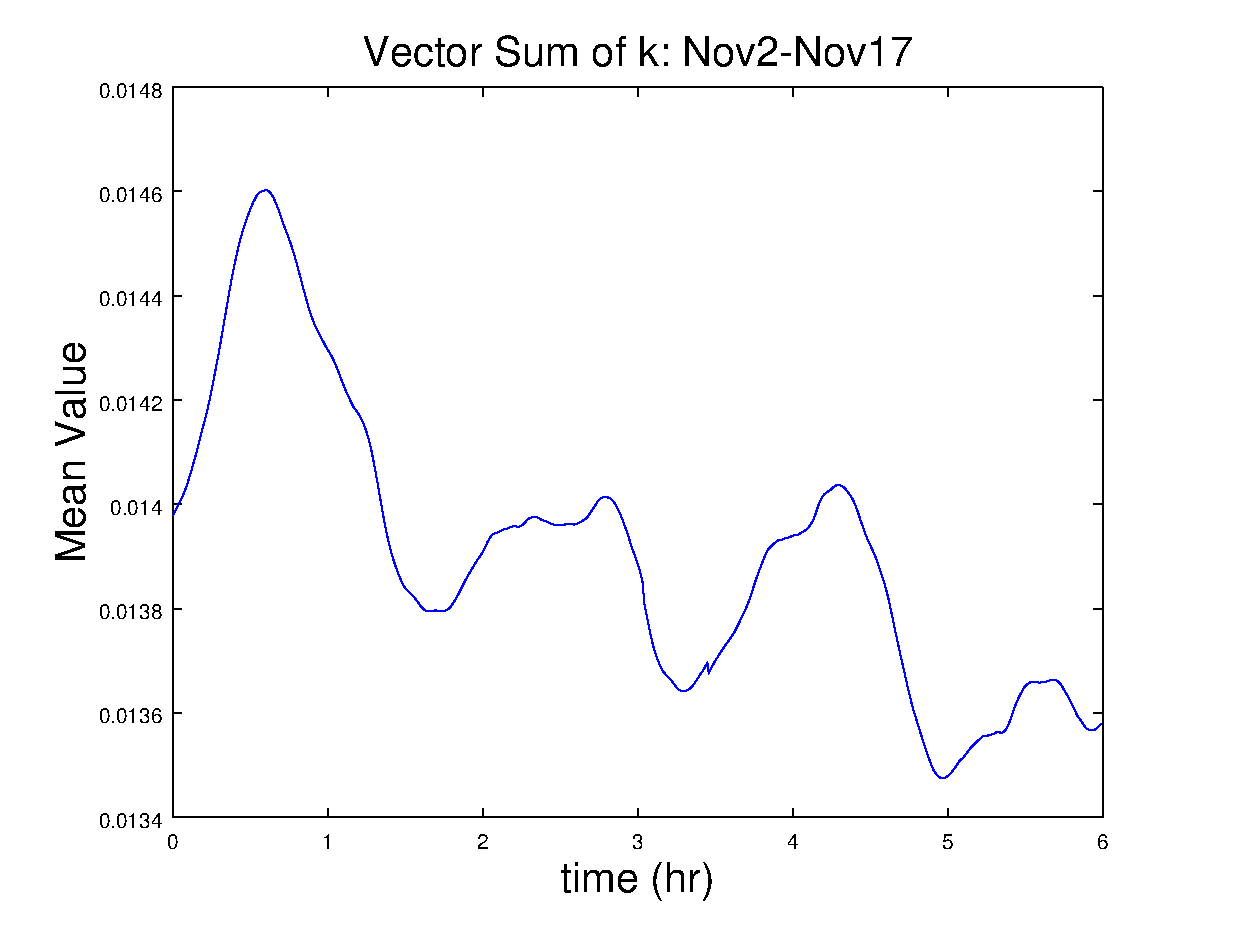
\includegraphics[width=0.5\textwidth]{../Datasets/Plots/VectorSumk}
	\caption{Mean Time Correlation vector $k$, Nov2 - Nov17, 2017}
	\label{fig:Ksum}
\end{figure}

Figure \ref{fig:SentShift} shows the sentiment shifted forward in the by $\tau_L$. It can be observed that 
rates of high change and local minima and maxima are matched between the two datasets. There are further similar plots 
Figure: \ref{fig:Dec23} - \ref{fig:Dec4-8} 

\begin{figure}[h]
	\centering
	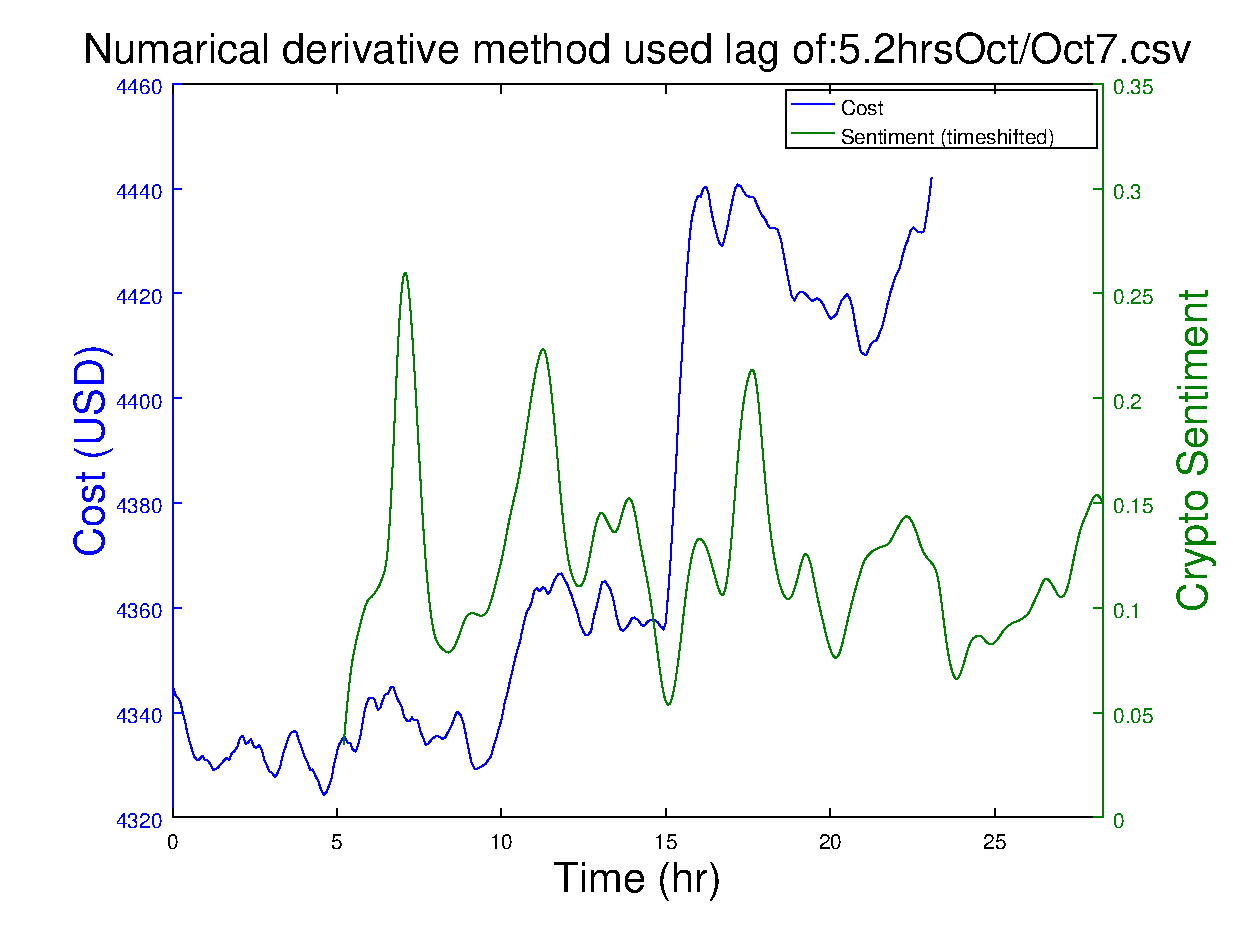
\includegraphics[width=0.5\textwidth]{../Datasets/Plots/Oct7_CostSen}
	\caption{Time Shifted Sentiment, October 9th 2017}
	\label{fig:SentShift}
\end{figure}

\subsection{Realtime Implementation}
Moving into a real time implementation was simple enough, previously the data post processing was being done in Octave, for the 
real time implementation Python was used. The application followed this structure,
\begin{enumerate}
	\item Fixed length of data was gathered, used 10hrs
	\item Steps above were executed, filtered, $k$ found and $\tau_L$ found
	\item Once $\tau_L$ was known, and you were at time $t = \tau$ you have $\tau - \tau_L$ worth of 'useful data' that you could
	make predictions on
	\item Buy and sell triggers were found (see below)
	\item Push notifications are sent to a mobile device using pushover \cite{Pushover}
\end{enumerate}
The crux of the real time application is finding the trigger points (Item 4), these are 
values or grouping of values that indicate that something is going to 
happen in $\tau_L$ time. As seen in Figure \ref{fig:SentShift} high slope values of sentiment can be used 
to infer changing cost values in time $\tau_L$. So high slope positive and negative slopes values were taken and
labeled as buy and sell triggers respectively, this is one possibly method of finding the triggers, but further work
should be done to understand if this is the best. 

This was the first crack at the real time app, it's currently running and sending out advice that is being used for HFT (high 
frequency trading)
\section{Future work}
\subsection{Optimisation problem}
There are a lot of parameters in the real time application that are in need of optimisation. 
\begin{itemize}
	\item $\tau$ - the amount of data to collect in the real time app before starting the post operations
	\item Number of buy/sell triggers, per $\tau$
	\item Stronger understanding of the Time Zone Inference (See appendix)
	\item Threshold for buy/sell triggers, what counts a 'high sentiment'
	\item Filter cutoff
\end{itemize}
Using all the archived data that we have been collecting over that past 5 months we could write an iterative application that
tunes each parameter to reduce the error. This would be extremely computational expensive most likely require offloading to
AWS or another similar service. 

\subsection{Machine Learning}
It's possible that there are correlations in the dataset that are not distinguishable by humans. Treating the problem
like a black box and using a deep neural net it might be possible to gain a deeper understanding of trends and stronger
correlations. In addition - we believe this is also a strong candidate for a Bayesian inference problem.

\subsection{Public Accessibility}
Conceivability all the work that has been done could be rolled into a pay to access platform that users can subscribe to help
make further informed trading decisions.

\section{Conclusion}
A lot is happening in the crypto currency landscape right now, as newly opened exchanges have given people access to invest in
the idea of a decentralised currency. This gives reason to believe that in addition to understanding 
the tech, it's also interesting to understand what people are thinking about the tech. This is important because the majority 
vote will determine the most widely adopted currency.\\

This was partially demonstrated in the work done above, but there's much more work that can be done . If we
are to better understand public perception methods other than just Twitter - we believe it's possible to see an ever better fit.
Aggregating a larger dataset could be used to understand the limitations of currencies and how volume spikes effect their
network. 

\section{Appendix}
\subsection{Time Zone Inferance}
There are also highly observable daily oscillations in tweet volume as seen in Figure \ref{fig:OSC}. 
These can be used to infer time zones of maximum influence.
\begin{figure}[h!]
	\centering
	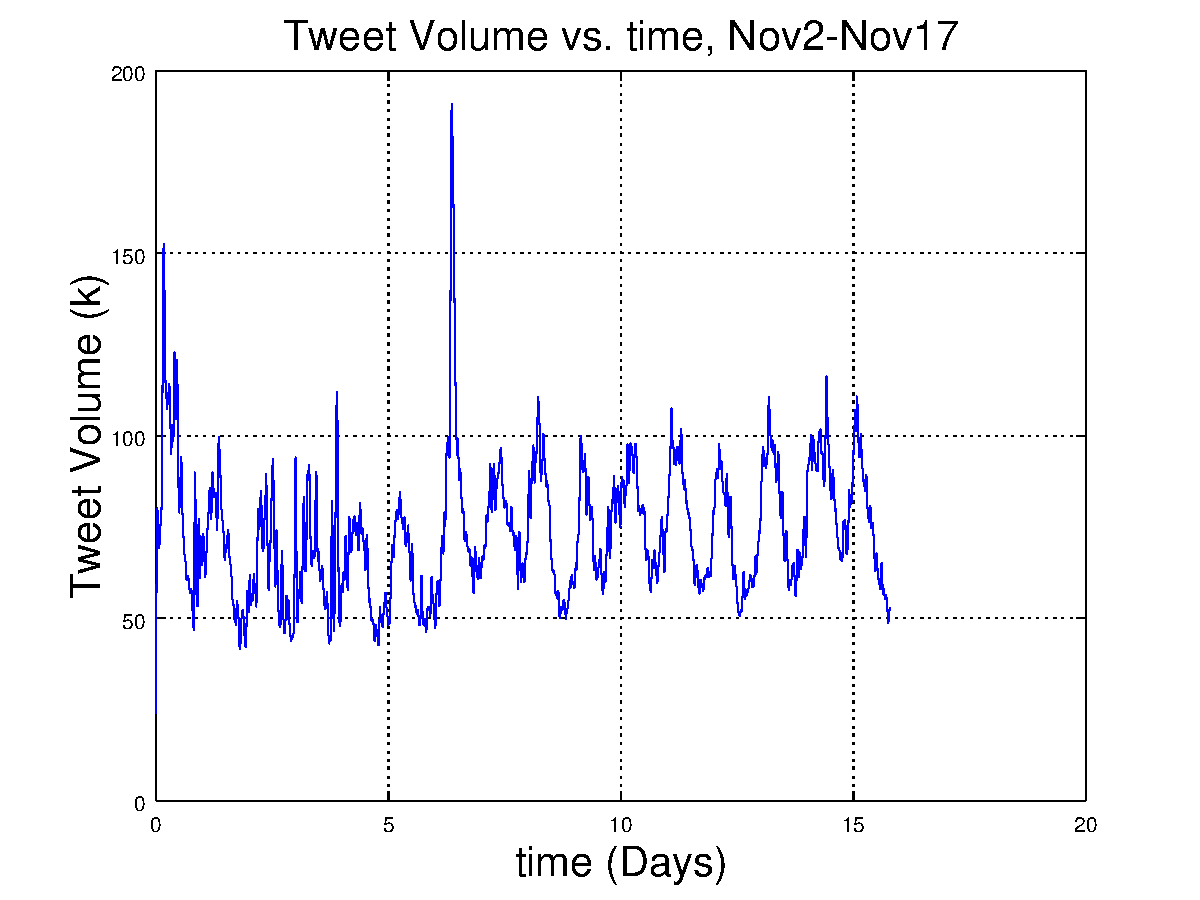
\includegraphics[width=0.5\textwidth]{../Datasets/Plots/TweetVolume}
	\caption{Tweet volume, Nov2 - Nov17, 2017}
	\label{fig:OSC}
\end{figure}

\subsection{Additional Data}

\begin{figure}[h!]
	\centering
	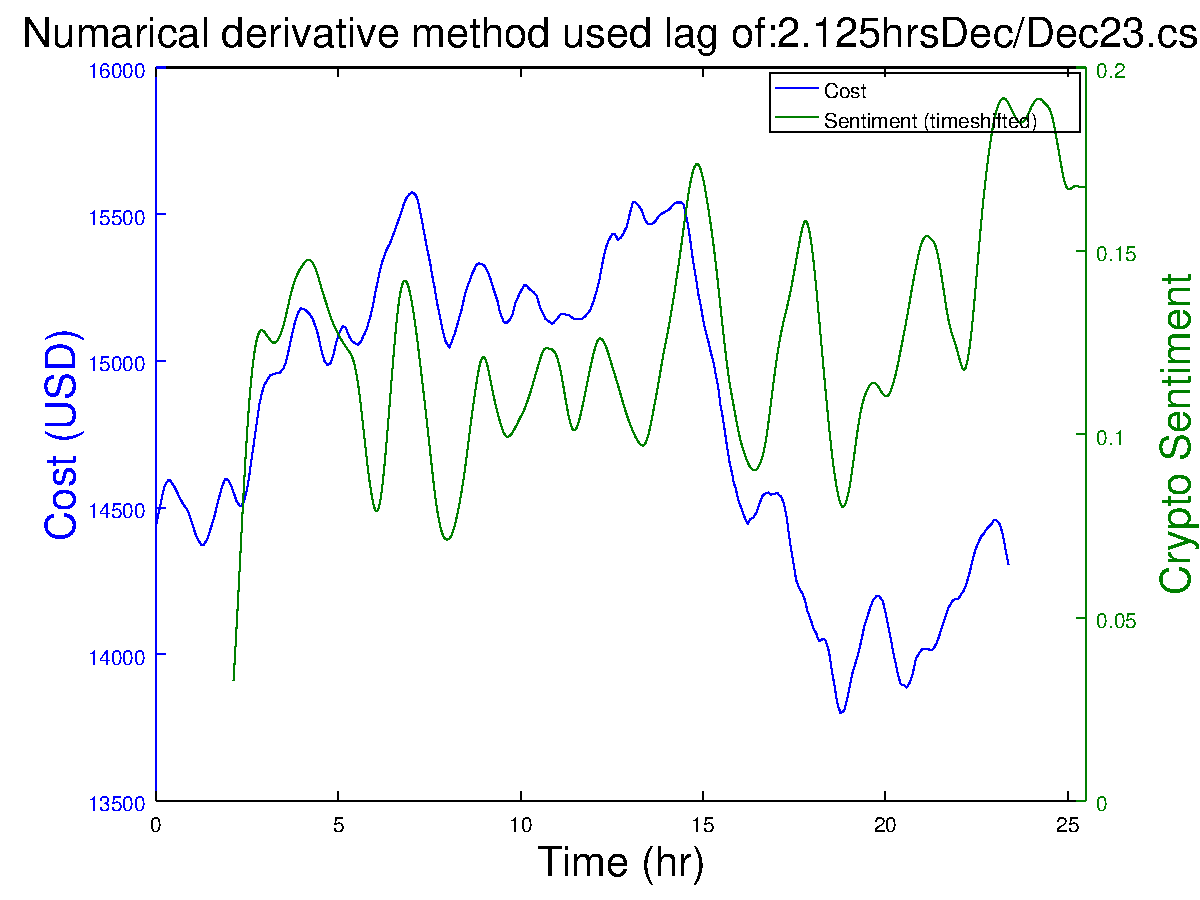
\includegraphics[width=0.5\textwidth]{../Datasets/Plots/Dec23}
	\caption{Dec23}
	\label{fig:Dec23}
\end{figure}

\begin{figure}[h!]
	\centering
	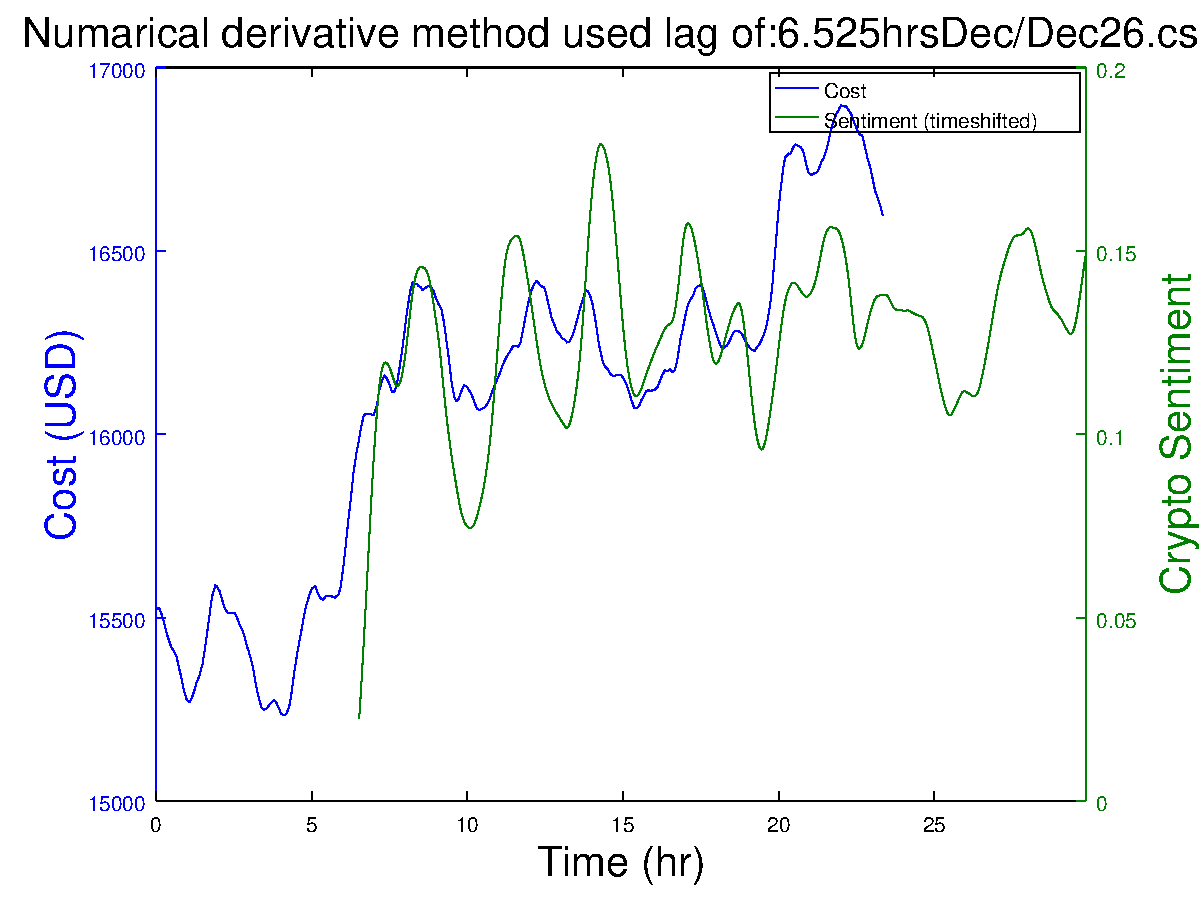
\includegraphics[width=0.5\textwidth]{../Datasets/Plots/Dec26}
	\caption{Dec26}
	\label{fig:Dec26}
\end{figure}

\begin{figure*}[h!]
	\centering
	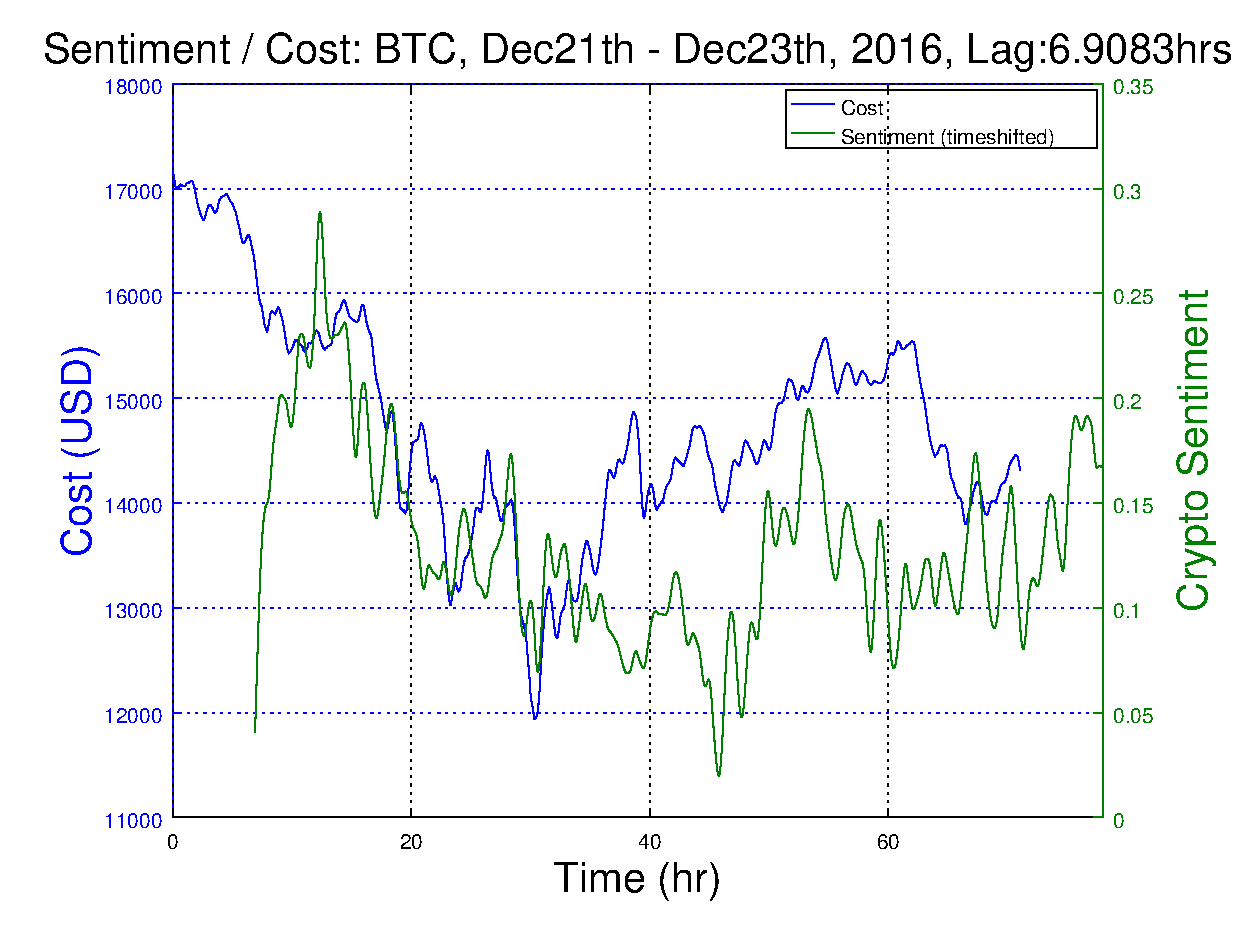
\includegraphics[width=0.8\textwidth]{../Datasets/Plots/Dec21-23}
	\caption{Bitcoin 'crash', Dec21 - Dec23, 2017}
	\label{fig:Dec21-23}
\end{figure*}

\begin{figure*}[h!]
	\centering
	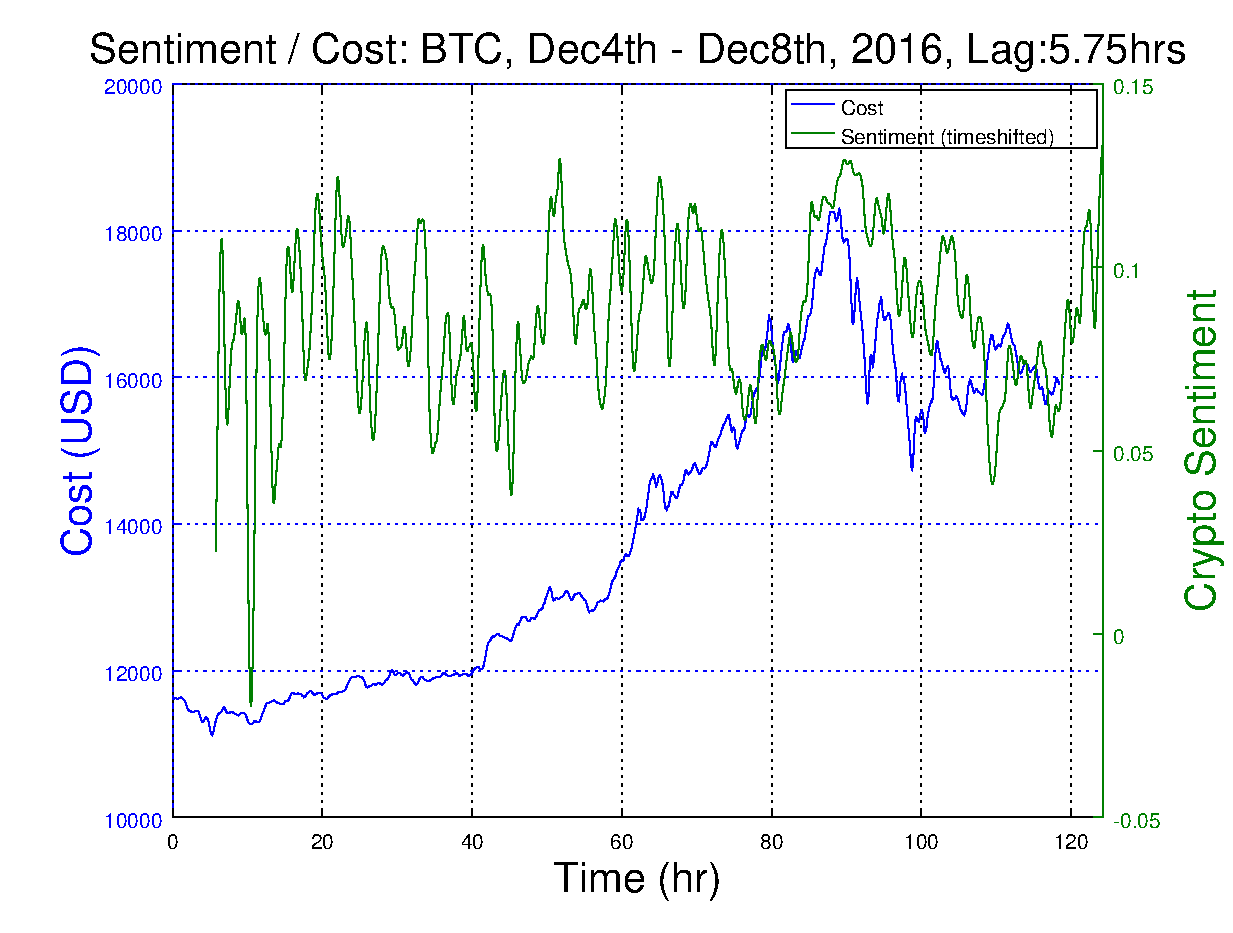
\includegraphics[width=0.8\textwidth]{../Datasets/Plots/Dec4-8}
	\caption{Four day trend - Dec4 - Dec8, 2017}
	\label{fig:Dec4-8}
\end{figure*}

\begin{thebibliography}{1}

\bibitem{BI1}
Anshul Mitta and Arpit Goel, \textit{Stock Prediction Using Twitter Sentiment Analysis}

\bibitem{Tweepy}
https://github.com/tweepy/tweepy

\bibitem{NLTK}
http://www.nltk.org/

\bibitem{Octave}
https://www.gnu.org/software/octave/

\bibitem{Pushover}
https://pushover.net/

\end{thebibliography}

\end{document}
